\chapter{Introduction}

  

\vspace{16pt}



Proof assistants are excellent tools for exploring the structure of mathematical proofs,
studying  which hypotheses are really needed, and which proof patterns are useful and/or
necessary. Since the development of a theory is represented as a bunch of computer files,
everyone is able to read the proofs with an arbitrary level of detail, or to play with the theory by building alternate proofs or definitions.


Among all the theorems proved with the help of proof assistants like \coq{}, \isabelle{}, \hol{}, etc.,
several statements and proofs  share some interesting features:
\begin{itemize}
\item Their statements are easy to understand, even by non-mathematicians
\item Their proof requires some non-trivial mathematical tools
\item Their mechanization on computer presents some methodological interest.
\end{itemize}


This is obviously the case of the four-color theorem~\cite{fourcolors}  and the Kepler conjecture~\cite{flyspeck2015}. We do not mention impressive works like the proof of the odd-order theorem ~\cite{oddorderthm}, since understanding its statement requires a quite good mathematical culture.




Hydra games (a.k.a. \emph{Hydra battles}) appeared in an article published in 1982 by two mathematicians:
L. Kirby and J. Paris~\cite{KP82}: \emph{Accessible Independence Results for Peano Arithmetic}. 
Although the mathematical contents of this 
paper are quite advanced, the rules of hydra battles are very easy to understand. There are now several sites on Internet where you can find tutorials on hydra games, together with simulators you can play with. See, for instance, the page written by Andrej Bauer~\cite{bauer2008}.



Hydra battles, as well as Goodstein Sequences~\cite{goodstein_1944, KP82}
are a nice way to present complex termination problems.
The article by Kirby and Paris presents a proof of termination
based on ordinal numbers, as well as a proof that this termination is not
provable in Peano arithmetic. In the book dedicated to 
J.P. ~Jouannaud \cite{HommageJPJ}, N.~Dershowitz and G.~Moser  give a thorough survey on this topic~\cite{Dershowitz2007}.



Here, we present a development  for the \coq{} proof assistant, after the work of Kirby and Paris. This formalization contains the following main parts:

\begin{itemize}
\item Representation in \coq{} of hydras and hydra battles
\item A proof that every battle is finite and won by Hercules. This proof is based on a \emph{variant} which maps any hydra to an ordinal strictly less than $\epsilon_0$ and is strictly decreasing along any battle.

\item Using a combinatorial toolkit designed by J.~Ketonen and R.~Solovay~\cite{KS81}, we prove that, for any ordinal $\mu<\epsilon_0$, there exists no such variant mapping any hydra to an ordinal stricly less than $\mu$. Thus, the complexity of $\epsilon_0$ is really needed in the previous proof.

\item We prove a relation between the length of a ``classic''  class of  battles
and the Wainer-Hardy hierarchy of ``rapidly growing functions'' $H_\alpha$~\cite{Wainer1970}. The considered class of battles, which we call \emph{standard}  is the most considered one in the scientific  litterature(including popularization).
\end{itemize}


Simply put, this document tries to combines the scientific interest of two articles~\cite{KP82, KS81} and a book~\cite{schutte} with the playful activity of truly proving theorems.
We hope  that such a work, besides exploring a nice piece of discrete maths, 
will show how \coq{} and its standard library are well fitted to help us to understand some non-trivial mathematical developments, and also to experiment the constructive parts of  the proof through functional programming.


\begin{figure}[h]
  \centering
  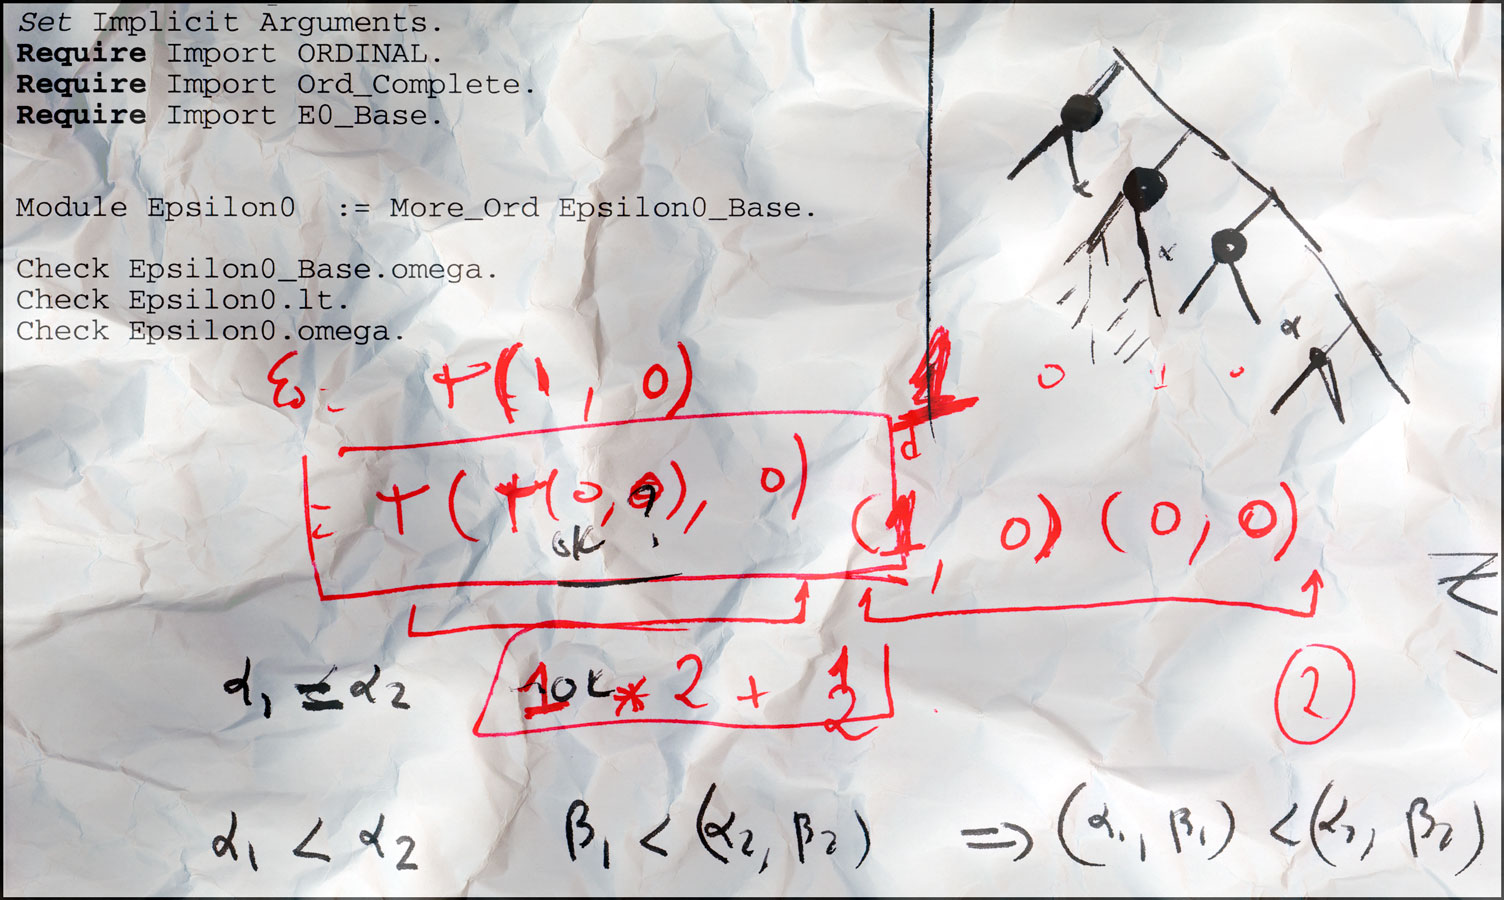
\includegraphics[width=11cm]{epsilon0.jpg}
  \caption{Discrete mathematics and formal proofs}
  \label{fig:gamma0}
\end{figure}
 We also hope to provide a little clarification on infinity (both potential and actual) through the notions of function, computation, limit,
 types and proofs.



\subsection*{Remarks}
In~\cite{KP82}, Kirby and Paris showed  that there is no proof of termination of all hydra battles in Peano Arithmetic (PA).
Since we are used to writing proofs in higher order logic, the restriction to PA was quite unnatural for us. So we chosed to prove another statement without any reference to PA, by considering a class of proofs indexed by ordinal numbers upto $\epsilon_0$.



Unlike mathematical literature, where definitions and proofs are spread over many articles and books,
the whole proof is now inside your computer. It is composed of the \texttt{.v} files you downloaded and 
parts of \coq's standard library. Thus, there is no ambiguity in our definitions and the premises of the theorems. Furthermore, you will be able to navigate through the development, using your favourite text editor or IDE, and some commands like \texttt{Search}, \texttt{Locate}, \texttt{Print Assumptions}, etc.

Except in the \texttt{Schutte} library, dedicated to an axiomatic presentation of the set of countable ordinal numbers, all our development is axiom-free, and respects the rules of intuitionistic logic. Note that we also use the \texttt{Equations} plug-in~\cite{sozeau:hal-01671777} for defining several rapidly growing hierarchy of functions, in Chap.~\ref{chap:alpha-large}. This plug-in imports the known-as-harmless following axiom:

\begin{Coqsrc}
FunctionalExtensionality.functional_extensionality_dep : 
forall (A : Type) (B : A -> Type) (f g : forall x : A, B x),
(forall x : A, f x = g x) -> f = g
\end{Coqsrc}



\paragraph*{Main references}

In our development, we adapt the definitions and prove many theorems which
we found in the following articles. 
\begin{itemize}
\item ``Accessible independence results for Peano arithmetic''  by Laurie Kirby and Jeff Paris~\cite{KP82}
\item ''Rapidly growing Ramsey Functions'' by Jussi Ketonen and Robert Solovay~\cite{KS81}
\item ``The Termite and the Tower'', by Will Sladek~\cite{Sladek07thetermite}
\item Chapter V of ``Proof Theory'' by Kurt Schütte~\cite{Schutte}
\end{itemize}



\subsubsection*{Structure of this document}
\begin{itemize}
\item Whenever several implementations are possible, we will discuss the pros and cons of every possible choice
\item Most of the proofs we present are \emph{constructive}. Whenever possible, we provide the user with an associated function, which she or he can apply in \gallina{} or \ocaml{} in order to get a ``concrete'' feeling of the meaning of the considered theorem.
For instance, in Chapter~\vref{chap:ketonen}, the notion of \emph{limit ordinal} is
made more ``concrete'' thanks to a function \texttt{canon} which computes every item of a sequence which converges on a given limit ordinal $\alpha$. This simply typed function allows the user/reader to make her/his own experimentations.
For instance, one can very easily compute the $42$-nd item of a sequence which converges towards $\omega^{\omega^\omega}$.


\item We found it interesting to present several  implementions of a given concept. After some discussions of the pros and cons of each solution, we will choose to develop only one of them, leaving the others  as exercises or projects (i.e., big or difficult exercises).
In order to discuss which assumptions are really needed for proving a theorem, we will also present 
several aborted proofs.

 \end{itemize}





\paragraph*{Warning:}

This document is \emph{not} an introductory text for \coq{}, and there are many aspects of this proof assistant that are not covered. 
 The reader should already have some basic experience with the \coq{} system. The Reference Manual and several tutorials are available on \coq{} page~\cite{Coq}.  First chapters of textbooks like \emph{Interactive Theorem Proving and Program Development}~\cite{BC04}, \emph{Software Foundations}~\cite{SF} or  \emph{Certified Programming with Dependent Types} ~\cite{chlipalacpdt2011} will give you the right background. 


\subsubsection*{State of the development}
The \coq{} scripts herein are in constant development since our contribution~\cite{CantorContrib} on ordinal notations for the ordinals $\epsilon_0$ and $\Gamma_0$.
We added new material : axiomatic definition of countable ordinals after Schütte~\cite{Schutte}, combinatorial aspects of $\epsilon_0$, after Ketonen and Solovay~\cite{KS81} and Kirby and Paris~\cite{KP82}, recent \coq{} technology: type classes, equations, etc.

We are now working in order to make clumsy proofs more readable, simplify definitions, 
to ``factorize'' proofs as much as possible. 

Many ``todo''s or projects are put in this text, suggesting possible improvements.

\subsubsection*{Contributions}
Many thanks to \'Evelyne Contejean and Florian Hatat for their contribution. \'Evelyne contributed libraries on the recusrive path ordering (\emph{rpo}) for proving the well-foundedness of our representation of $\epsilon_0$ and $\Gamma_0$.
Florian Hatat proved many useful lemmas on countable sets, which we used in our adaptation of Schütte's formalization of countable ordinals.



\label{sec:orgheadline2}

Any form of contribution  is welcome: correction of errors, improvement of
Coq scripts, proposition of inclusion of new chapters, and generally any
comment or proposition that would help us. The text contains several \emph{projects} which, when completed, may improve the present work.
Please do not hesitate to bring your contribution!



\subsubsection*{Acknowledgements}
\label{sec:orgheadline5}
    Many thanks to David Ilcinkas, Sylvain Salvati, Alan Schmitt and Théo Zimmerman for their help on the elaboration of this document, and to the
 members of the \emph{Formal Methods} team at laBRI for their helpful comments 
on an oral presentation of this work. 

Many thanks also to the Coq development team, Yves Bertot, and members of the \emph{Coq Club} for interesting discussions about the \coq{} system and the Calculus of Inductive Constructions.

The author of the present document wishes to express his gratitude to the late Patrick Dehornoy, whose talk  was determinant for our desire to work on this topic.

I owe my interest in discrete mathematics and their relation to formal proofs and functional programming  to Srecko Brlek.  Equally, there is W. H. Burge's book ``\emph{Recursive Programming Techniques}'' ~\cite{burge} which was a great  source of inspiration.

\subsection*{Typographical conventions}

Quotations from our  \coq{} source are displayed as follows:


  \begin{Coqsrc}
 Require Import Arith.

 Definition square (n:nat) := n * n.

 Lemma square_double : exists n:nat, n + n = square n.
 Proof.
    exists 2. 
  \end{Coqsrc}

Answers from \coq{} (including sub-goals, error messages, etc.) are displayed in slanted style
with a different background color.



 \begin{Coqanswer}
 1 subgoal, subgoal 1 (ID 5)
  
  ============================
   2 + 2 = square 2
   
 \end{Coqanswer}

 \begin{Coqsrc}
   reflexivity.
Qed.
 \end{Coqsrc}

\subsection*{Alternative or bad definitions}

Finally, we decided to include definitions or lemma statements, as well as tactics,  that lead to
dead-ends or to too complex developments, with the following coloring.
Bad definitions 
 and encapsulation in modules called \texttt{Bad}, \texttt{Bad1}, etc.


 \begin{Coqbad}
Module Bad.

Definition double (n:nat)  := n + 2.
 
Lemma lt_double : forall n:nat, n < double  n.
Proof.
   unfold double; omega.
Qed.

End Bad.
  \end{Coqbad}

Likewise, alternative, but still unexplored definitions will be presented in modules
\texttt{Alt}, \texttt{Alt1}, etc. Using these definitions is left as an implicit exercise.


\begin{Coqalt}
Module Alt.

  Definition double (n : nat) := 2 * n.

End Alt.
\end{Coqalt}

\begin{Coqsrc}
Lemma alt_double_ok n : Nat.double n = Alt.double n.
Proof.
  unfold Alt.double, Nat.double.
  omega.
Qed.
\end{Coqsrc}

% \subsubsection{Links to the Coq source}

% Active links towards our \coq{} modules may be incorrect if you got this \texttt{pdf} document otherwise than by compiling the distribution available in
% \url{http://www.labri.fr/casteran/CoqArt/le_teaser/Teaser.tar.gz}.




